\documentclass[11pt]{article}
% Defining all packages that are used in this document
\usepackage[utf8]{inputenc}
\usepackage[english]{babel} % Change this to norwegian if report is written in norwegian
\usepackage{amsmath}   % Package for math files
\usepackage{parskip}   % No indent, but instead paragraphs
\usepackage{graphicx}  % Place figures
\usepackage{caption}   % Place captions in tables and figures
\usepackage{subcaption}% 
\usepackage{subfiles}  % 
%\usepackage{subfigure}
\usepackage{pdfpages}
\usepackage[T1]{fontenc} 
\usepackage[euler]{textgreek} % To get greek letters as we know them
\usepackage{amssymb}   % 
\usepackage{placeins}  % \FloatBarrier so figures can't float beyond some point in text
\usepackage{fullpage}  % Uses more of the page
\usepackage{float}     % Able to make figures and tables float \begin{figure}[H] to keep them HERE
\usepackage[version=4]{mhchem} % \ce{} to write chemical eq.
\usepackage{siunitx}   % Ex: \si{\meter\per\square\second}
\usepackage{booktabs}  % Behind-the-scenes optimization of tables. \toprule, \midrule, \bottomrule
\usepackage{multirow}
\usepackage{hyperref}  % Ability to click on references like equations, figures, sections etc. \ref{eq:my_eq} clickable

%表格自动生成
\renewcommand {\thetable} {\thechapter{}.\arabic{table}}
%表格根据章节自动命名
\renewcommand {\thefigure} {\thechapter{}.\arabic{figure}}
%图片根据章节自动命名
\numberwithin{figure}{section}
\numberwithin{table}{section}
\numberwithin{equation}{section}
%以上三个皆控制重命名

\usepackage{fontspec}
\setmainfont{Arial}

\hypersetup{
    colorlinks,
    citecolor=black,
    filecolor=black,
    linkcolor=black,
    urlcolor=black
}
\iffalse
\usepackage{fancyhdr}
	%fancyhdr:一个很强大的宏包,用于自定义设计页面风格并命名以供调用。
	\pagestyle{fancy}
	%\rhead{实验B16 基于vLight的光学仿真基础实验}
	%\lhead{基础物理实验\uppercase\expandafter{\romannumeral2}实验报告}
	\cfoot{ \thepage}  %当前页
	\rfoot{\today}
		%分别是右页眉、左页眉、中页脚、右页脚
	\renewcommand{\headrulewidth}{0pt}
	%\renewcommand{\theenumi}{(\arabic{enumi})}
\fi

\usepackage[autolinebreaks,useliterate,numbered]{mcode} % Ability to paste smooth MATLAB code
\newcommand{\figref}[1]{\figurename~\ref{#1}} %Nice reference to figures
%\linespread{1}
\usepackage{setspace}
\setstretch{1.2}
%\renewcommand{\baselinestretch}{1.5}
\title{
    Robotics design challenge  \\
    (MATLAB/SIMULINK)}
\author{
	Jiaqi, Yao. Ruixin, Zhan. Xuzhao, Zhang. Xiaoyu, Zhang%\footnote{jy431@exeter.ac.uk}
}
%\date{  \today}

\begin{document}
\maketitle
%\begin{abstract}

%\end{abstract}
\pagenumbering{gobble} % Turn off page numbering
%\newpage
%\tableofcontents
%\newpage
\pagenumbering{arabic} % Turn on normal pagenumbering
%%%%%%%%%%%%%%%%%%%%%%%%%%%%%%%%%%%%%%%%%%%%%%%%%%%%%%%%%%
% Main contents - Do NOT write your text in main.tex! Use                     the tex files in the folders below
\section{Brief report}

	\noindent Dear Officer:
	
	\noindent We understand that you are looking for a welding robot for the automotive industry and our team has found our product to be the right fit for your needs. I will then briefly describe our robot and show its advantages in terms of design and precision.
	
	\noindent We have designed a four-armed robot according to your requirements and have considered its parameters, which you can see in Table 1 and Table 2. After simulation analysis, this design is reasonable and can perform the task accurately in the working area. We have also created a kinematic diagram (Figure 2.1) and a workspace diagram (Figure 3.1)
	
	\noindent The maximum error in end effector position on the x and z axes is below 0.05, while the maximum error on the y axis is slightly This shows the amazing accuracy of the robot in its movements and workings. You can see the specific images of the errors in Figure 1 and Figure 2.

\section{Introduction}
\FloatBarrier % Now figures cannot float above section title

Our product is a type of mechanical equipment used for automated welding. Our robotic arm can be widely used in various welding operations in the manufacturing industry, including automotive manufacturing, aerospace, construction, and manufacturing.

Our product has many adavantages. Firstly, it can improve production efficiency and quality by reducing the negative impact of human factors on production through automated welding operations. Secondly, it can reduce the danger of the work environment. 

In summary, the four-arm welding robot is an efficient and accurate welding device with many advantages. It will become an important part of automated production in the manufacturing industry, providing a reliable solution for various production operations.









\iffalse
The purpose of this experiment is to investigate the behaviour of a mild steel portal frame model when subjected to increasing loads.

The rig consists of a loading system that applies a vertical load at the center of the beam and a horizontal load at the top of one column. As shown in \autoref{f0}.

\begin{figure}[htbp]
    \centering
    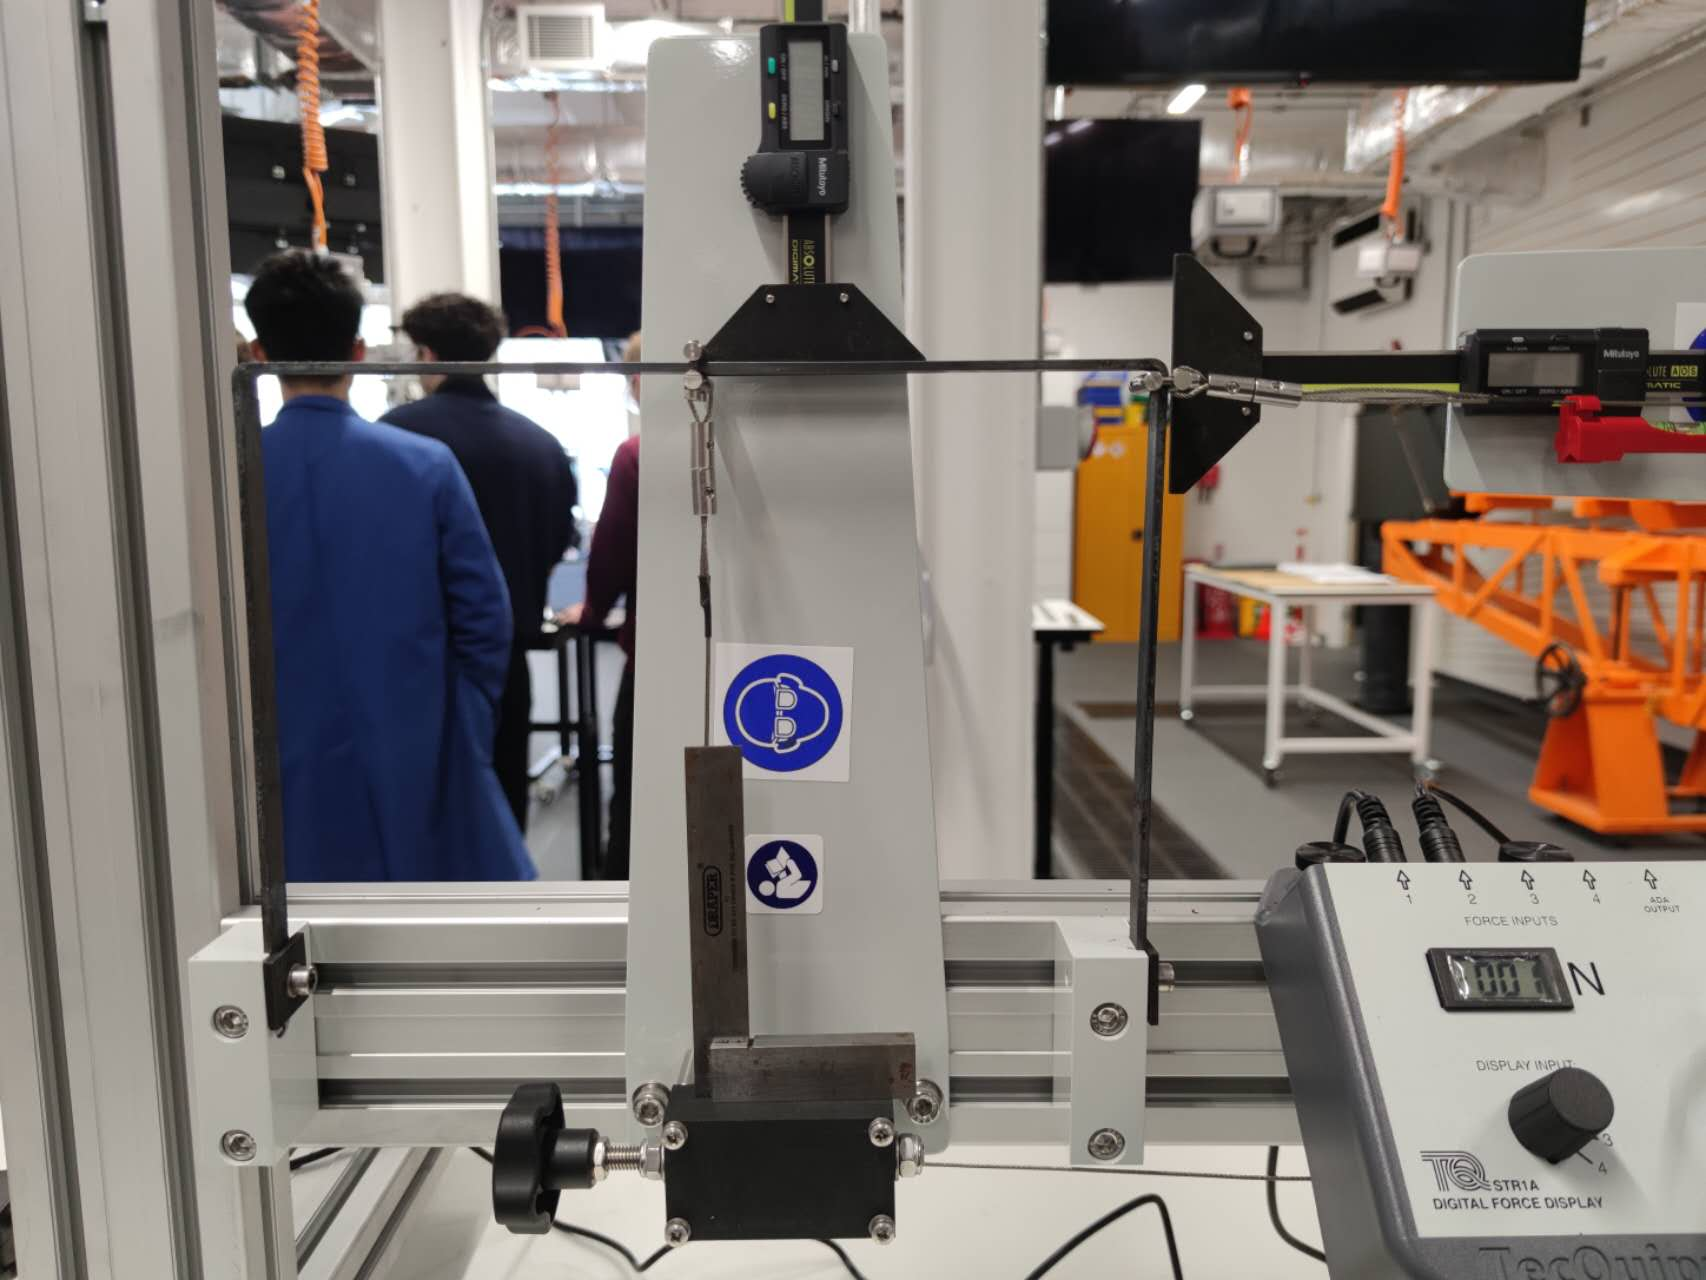
\includegraphics[width=7.5cm]{./fig/00.jpg}
    \caption{Experimental procedure}
    \label{f0}
\end{figure}

\fi



\section{Task 1}
\FloatBarrier % Now figures cannot float above section title


\subsection{Originality and uniqueness of the robot}

Our robot's uniqueness lies in the fact that it is a four-arm robot. Although two-arm and three-arm robots can perform the same tasks, they are relatively unstable and more difficult to control. In addition, a four-arm robot can provide a larger workspace and a greater potential for improvement.

\subsection{Property of all the arms and the joints}

We have designed 4 joints for the robot, 2 of which are revolute type and 2 are prismatic type. At the same time, there are four corresponding robotic arms, whose parameters are shown in the Table \ref{T 2.1} and Table \ref{T 2.2}

\begin{minipage}[htbp]{\textwidth}
    \makeatletter\def\@captype{table}
    \centering
    \scalebox{1}{
    \begin{tabular}{cccc}
    \hline
    Name & Body Mass (kg) & Center of mass & Inertia ($I_{xx}$ $I_{yy}$ $I_{zz}$) ($kg \cdot m^2$)                  \\ \hline
    R1   & 10        & (0 0 0)        & (0.27 0.27 0.8 )     \\
    R2   & 10        & (0 0 0)        & (0.27 0.27 0.8 )     \\
    P1   & 1.5       & (0 0 0)        & (0.07 0.07 0.07 )    \\
    P2   & 1.5       & (0 0 0)        & (0.07 0.07 0.07 )    \\
    Tool & 1.2       & (0 0 0)        & (0.002 0.002 0.004 ) \\ \hline
    \end{tabular}} 
    \caption{Robot arm parameters}
    \label{T 2.1} 
\end{minipage}


\begin{minipage}[htbp]{\textwidth}
    \makeatletter\def\@captype{table}
    \centering
    \scalebox{1}{
    \begin{tabular}{cccc}
    \hline
    Joint & Type & Position Limit (rad \& m) & Joint Axis                   \\ \hline
    1   & revolute       & $[-5\frac{\pi}{180}, 5\frac{\pi}{180}]$ & [0 0 1]     \\
    2   & revolute       & $[-30\frac{\pi}{180}, 30\frac{\pi}{180}]$        & [0 1 0]     \\
    3   & prismatic      & $[-0.5,0.5]$        & [1 0 0]    \\
    4   & prismatic      & $[-1, 1]$        & [0 1 0]    \\ 
    Fixed &revolute & N/A & N/A \\\hline
    \end{tabular}} 
    \caption{Joint parameters}
    \label{T 2.2} 
\end{minipage}

Figure \ref{F 2.1} is a schematic diagram of the robot in MATLAB.
\begin{figure}[htbp]
    \centering
    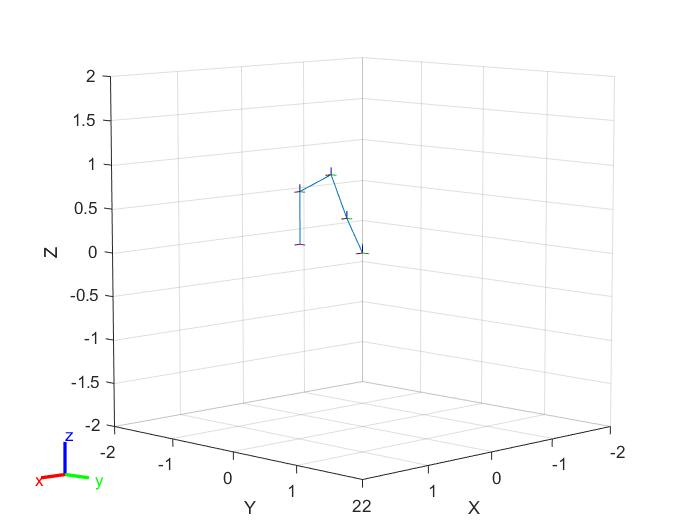
\includegraphics[width=7cm]{./fig/1.jpg}
    \caption{Robot schematic}
    \label{F 2.1}
\end{figure}

\subsection{Collision discussion}

Our designed robot is free from collisions. In most cases, collisions occur on the two arms of the rotating joints whose rotation angle is greater than $±90^\circ$. For our designed robot, the total range of motion for the two movable joints is $±35^\circ$, so there is no collision. Additionally, the animation of the robot's movement trajectory can be viewed in the dynamic image in Figure 8.

\section{Task 2}
\FloatBarrier % Now figures cannot float above section title

Here are the reachable workspace for the robot designed in Task 1.


\begin{figure}[htbp]
    \centering
    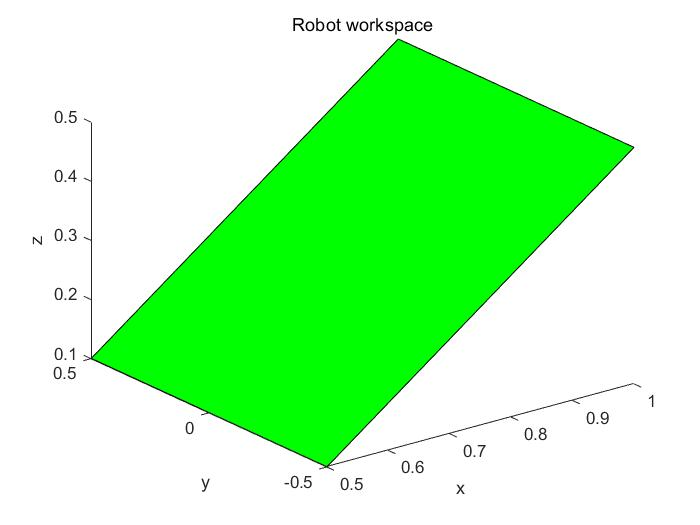
\includegraphics[width=10cm]{./fig/workspace.jpg}
    \caption{Experimental results}
    \label{f5}
\end{figure}



\newpage
\iffalse
The method of calculating the plastic moment is introduced in the powerpoint of the Week 6 lecture. As shown in the figure below \autoref{f1}.

\begin{figure}
    \centering
    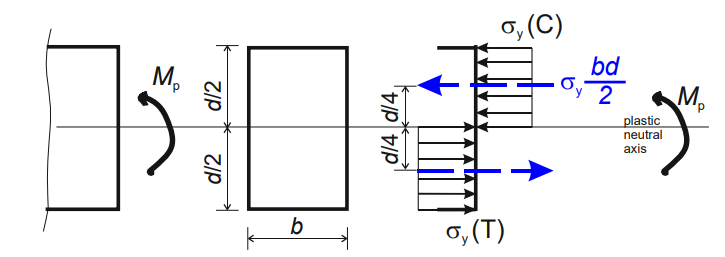
\includegraphics[width=10cm]{./fig/11.png}
    \caption{plastic modules of rectangular section  }
    \label{f1}
\end{figure}

The plastic moment $M_p$ when all points in the section reached
yield stress $\sigma_y(250Mpa)$ is caculated by:

\begin{equation} 
    M_p=\sigma_y\frac{bd}{2}(\frac{d}{4}+\frac{d}{4})
    \label{e1}
\end{equation}

Calculated from the data from \autoref{t1}, we get $M_p=8.67N \cdot m$.

There are three cases of collapse of plasticity of portal frame. We use virtual work method to caculate it.

\begin{figure}[htbp]
    \centering
    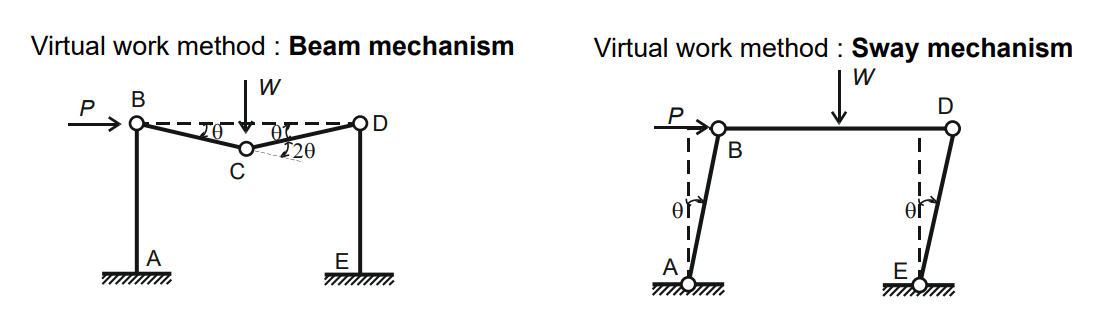
\includegraphics[width=10cm]{./fig/12.png}
    %\caption{plastic modules of rectangular section  }
    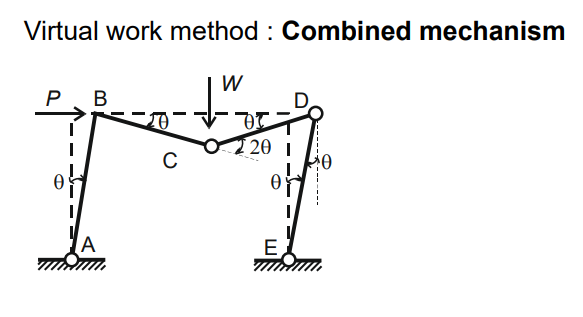
\includegraphics[width=5.5cm]{./fig/13.png}
    \caption{Three cases of collapse of plasticity of portal frame}
    \label{f2}
\end{figure}


$\bullet$ \textbf{Beam mechanism:} If $W>>P$, the hinges are likely to appear in B, C and D.



$\bullet$ \textbf{Sway mechanism:} If $P>>W$, the hinges are likely to appear in A, B, D and E.




$\bullet$ \textbf{Combined mechanism:} If P $\approx$ W, the smallest moment
is at B (as moments due to P
and W oppose each other), so
hinges form at other possible
locations. (The angle between ABC is $90^\circ$)

The virtual work method is: 

\begin{equation}
    \sum_i^{}{P_i\delta_i}=\sum_j^{}{M_j\theta_j}
    \label{e2}
\end{equation}

We noticed that the height (200mm) is equal to $\frac{2}{3}$ length (300mm). i.e. $H=\frac{2}{3}L$.

By using \autoref{e2}, we can get

$$
\left\{ \begin{array}{l}
	W\frac{\theta L}{2}=M_p\theta+M_p2\theta+M_p\theta \rightarrow W=\frac{8M_p}{L} (Beam)\\
	P\frac{2L}{3}\theta=M_p\theta+M_p\theta+M_p\theta+M_p\theta \rightarrow P=\frac{6M_p}{L} (Sway)\\
	P\frac{2L}{3}\theta+W\frac{\theta L}{2}=M_p\theta+M_p2\theta+M_p2\theta+M_p\theta \rightarrow 4P+3W=\frac{36M_p}{L} (Combined)\\
\end{array} \right. 
$$

Plot the relationships P-W on a graph

\begin{figure}[htbp]
    \centering
    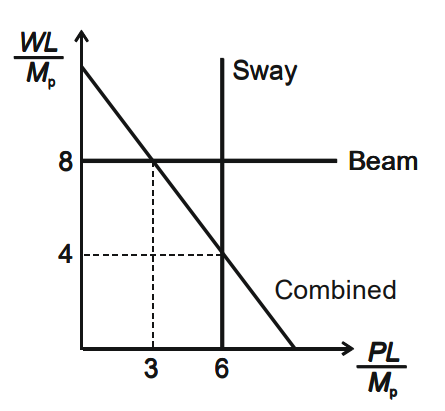
\includegraphics[width=6.5cm]{./fig/14.png}
    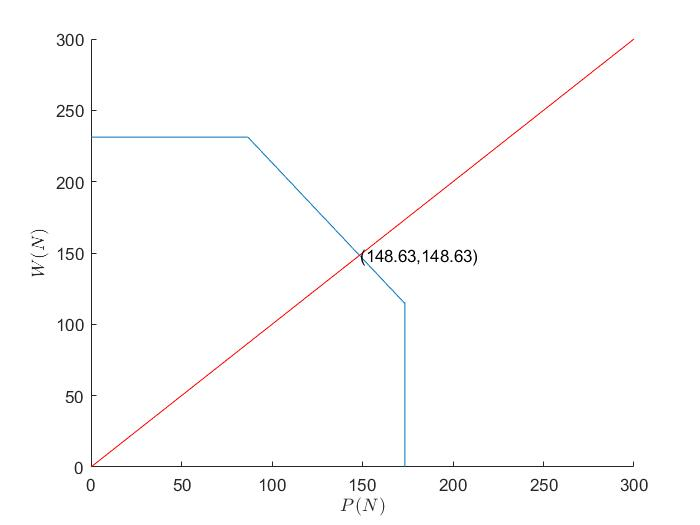
\includegraphics[width=8.5cm]{./fig/15.jpg}
    \caption{P-W graph}
    \label{f3}
\end{figure}



Substitude data from \autoref{t1} and \autoref{e1}, We have $\frac{M_p}{L}=28.9N$ and the boundary of the graph.

$$
\left\{ \begin{array}{l}
	W=\frac{8M_p}{L}=231.2\\
	P=\frac{6M_p}{L}=173.4\\
	4P+3W=\frac{36M_p}{L}=1040.4\\
\end{array} \right. 
$$

Plotting the three boundary lines with the applied load lines ($y=x$) on the graph, the following figure is obtained.

$$
\left\{ \begin{array}{l}
	4P+3W=1040.4\\
	P=W\\
\end{array} \right. 
$$
The solution to the equation is ($P=W=148.63(N)$)
where the coordinates of the load line and the boundary line are (148.63,148.63\label{ee}).


\fi





\section{Task 3}
\FloatBarrier % Now figures cannot float above section title

Here are the drawing of the kinematic diagram using the Denevit-Hartenberg frame rules for the robot designed in task 1.

\begin{figure}[htbp]
    \centering
    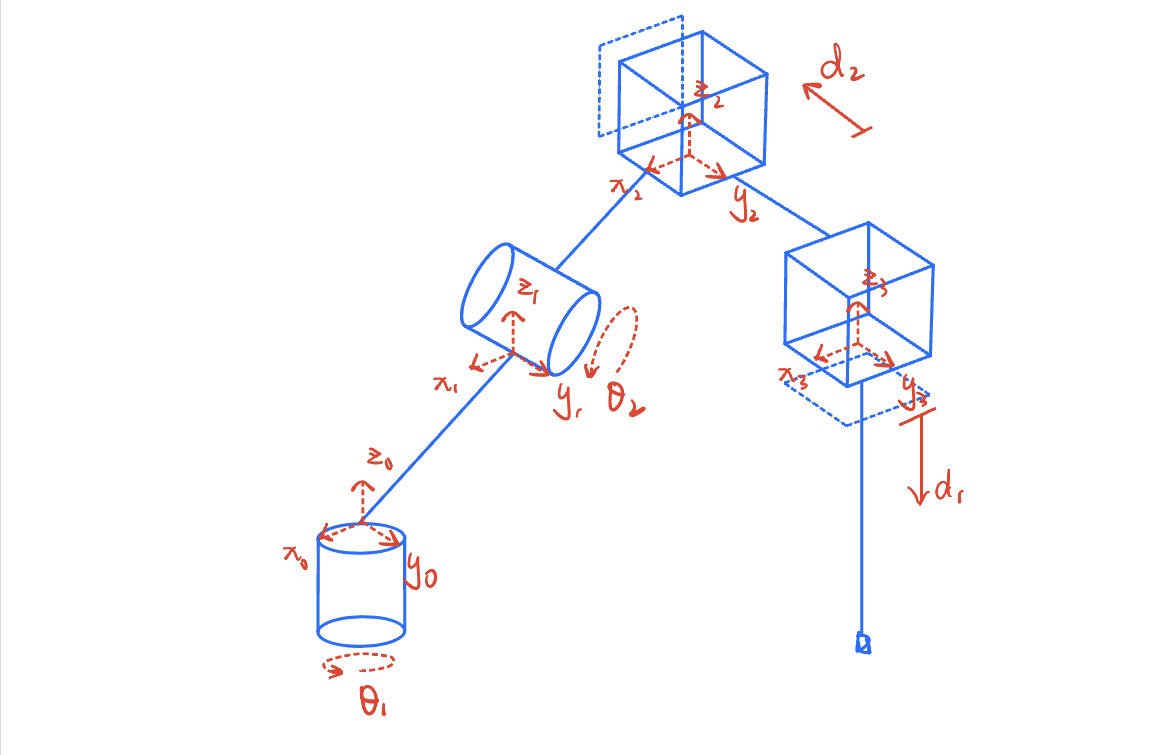
\includegraphics[width=7cm]{./fig/D-H.jpg}
    \caption{Experimental results}
    \label{f5}
\end{figure}


\section{Task 4}
\FloatBarrier % Now figures cannot float above section title


\subsection{Simulink}

\begin{figure}[htbp]
    \centering
    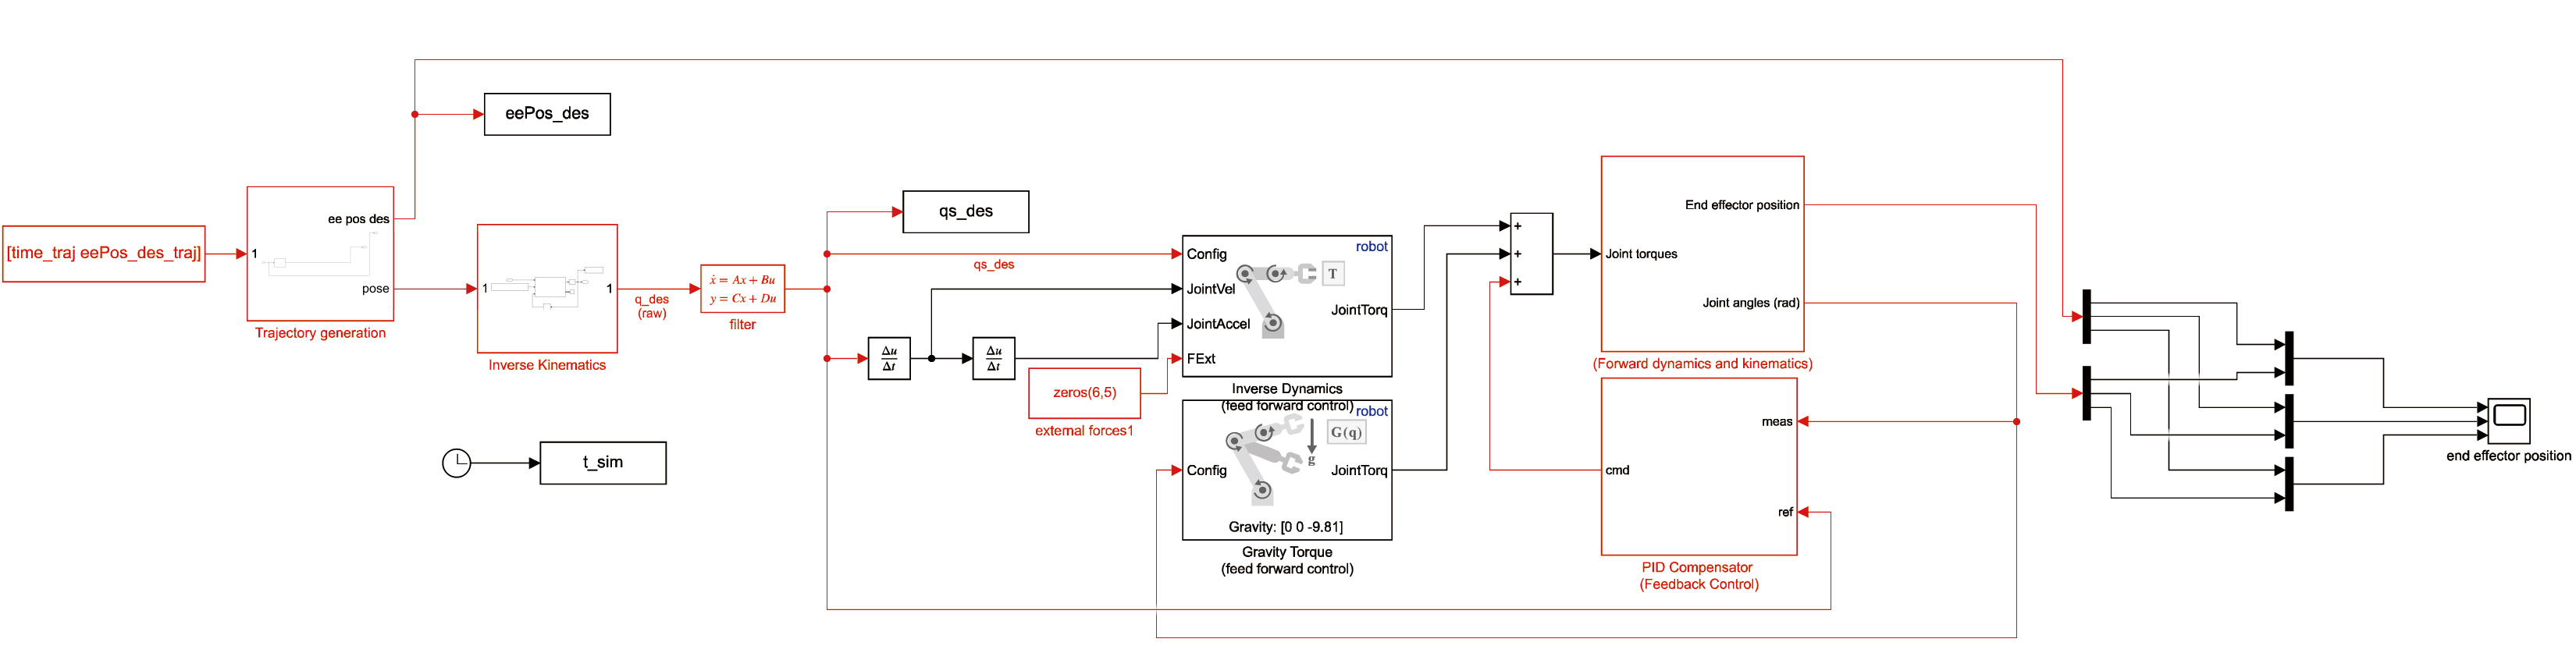
\includegraphics[width=17cm]{./fig/sim.jpg}
    \caption{plastic modules of rectangular section  }
    \label{f1}
\end{figure}

\subsubsection*{Tidy of the model}
To ensure aesthetic appeal, a modular design approach was adopted, where different modules represent different functionalities, thereby making the overall model's operation flow appear clear and concise.

\subsubsection*{Trajectory generation}

\begin{figure}[htbp]
    \centering
    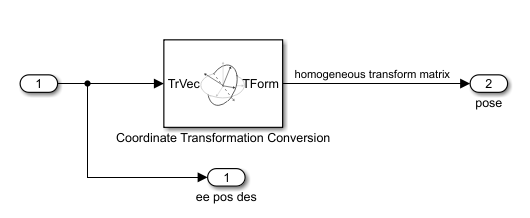
\includegraphics[width=8cm]{./fig/traj.png}
    \caption{plastic modules of rectangular section  }
    \label{f1}
\end{figure}

Trajectory generation module is an important component of robot motion planning, as it allows robots to move safely and efficiently in complex environments.This module is to convert signals from one coordinate system to another so that we can have easier control of the system. Additionally, the trajectory needs to be smooth, so that the robot does not make sudden changes in direction or speed that may destabilize the system or cause discomfort to human users.

We first calculate the path coordinate points and time series from the code, and use them as input parameters for trajectory calculation. Through trajectory calculation, we can obtain the expected end-effector position and the motion trajectory data applicable to each point after coordinate transformation (which is a 4001*3 data, recording the three-dimensional coordinate points of the path every 0.01 seconds and simulated for a total of 40 seconds).


\subsection{PID design}

\begin{figure}[htbp]
    \centering
    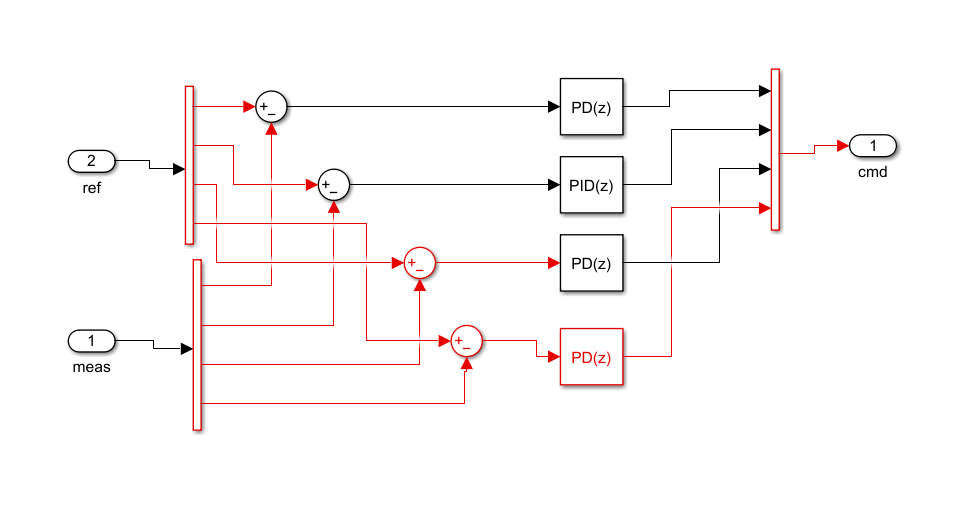
\includegraphics[width=10cm]{./fig/PID.png}
    \caption{plastic modules of rectangular section}
    \label{f1}
\end{figure}


With the aim of having better accruacy of the end effect position, we add a feedback control module. Feedback control is a control technique used in engineering to control a system by adjusting its behavior based on measured output signals. In feedback control, the output of the system is measured and compared to a desired end effect position. The difference between the measured output and the desired end effect position is called the error signal, which is then used to adjust the system's behavior through a feedback loop.

In the PID control module, we subtract the desired data from the actual data to obtain the error value, which is then used for PID calculation. We noticed that joints 1, 3, and 4 only use PD controllers because these three joints require a fast response speed and low overshoot, and have lower requirements for steady-state error. For joint 2, which uses a PID controller, it is sensitive to steady-state error due to its rotation around the y-axis. Although there may be difficulty in tuning, we successfully completed the debugging process.


\subsection{Results}

\begin{figure}[htbp]
    \centering
    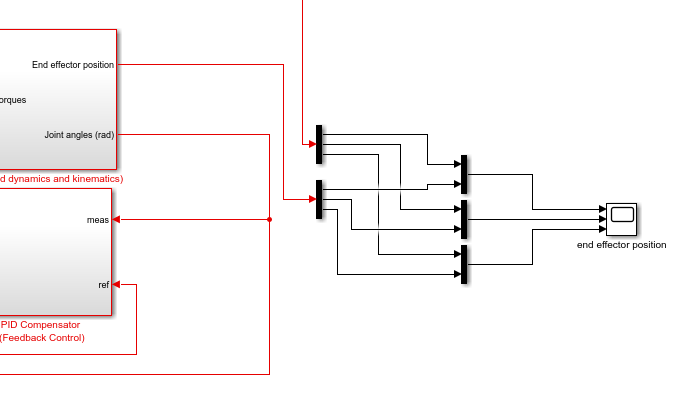
\includegraphics[width=7cm]{./fig/re.png}
    \caption{plastic modules of rectangular section}
    \label{f1}
\end{figure}

Finally, set the end effector positions and the desired end effector positoins as the input, draw the plot with their x y z positions followed by the time respectively.

\subsubsection*{Input torque}

\begin{figure}[htbp]
    \centering
    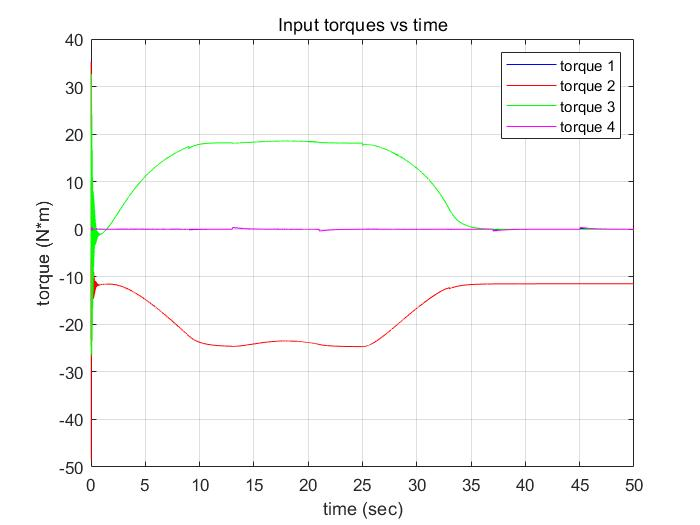
\includegraphics[width=10cm]{./fig/3.jpg}
    \caption{plastic modules of rectangular section}
    \label{f1}
\end{figure}


\subsubsection*{Joint angle}

\begin{figure}[htbp]
    \centering
    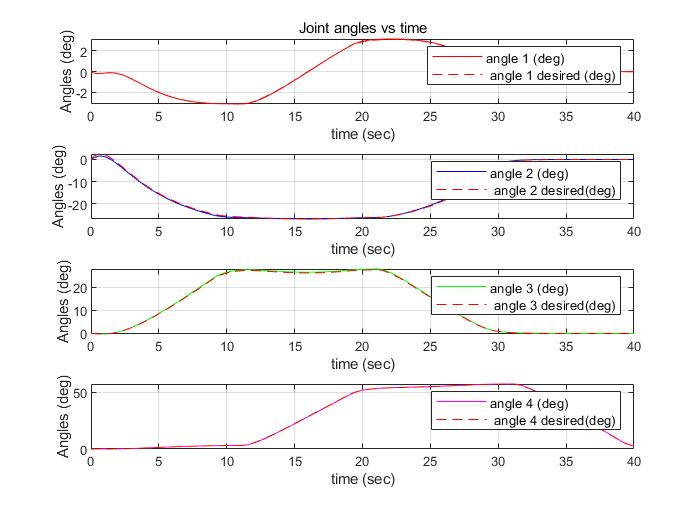
\includegraphics[width=8cm]{./fig/4.jpg}
    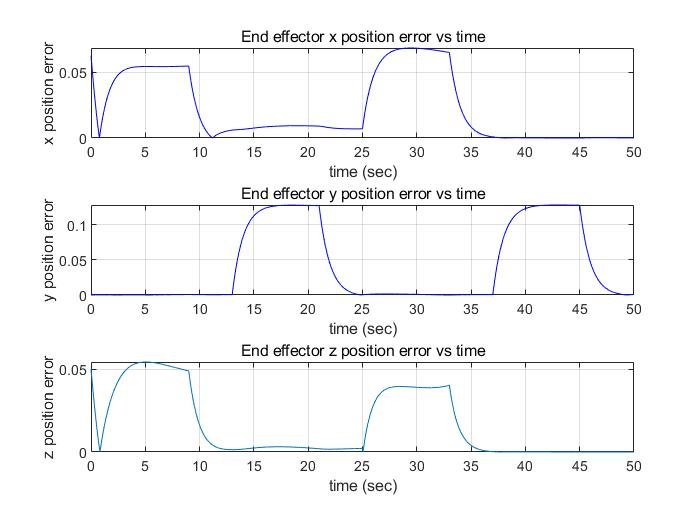
\includegraphics[width=8cm]{./fig/6.jpg}
    \caption{plastic modules of rectangular section}
    \label{f1}
\end{figure}

\subsubsection*{End Effector Position}

\begin{figure}[htbp]
    \centering
    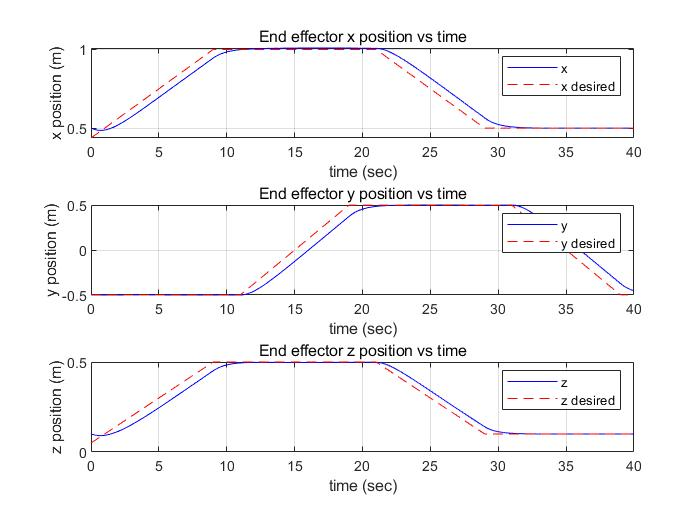
\includegraphics[width=8cm]{./fig/5.jpg}
    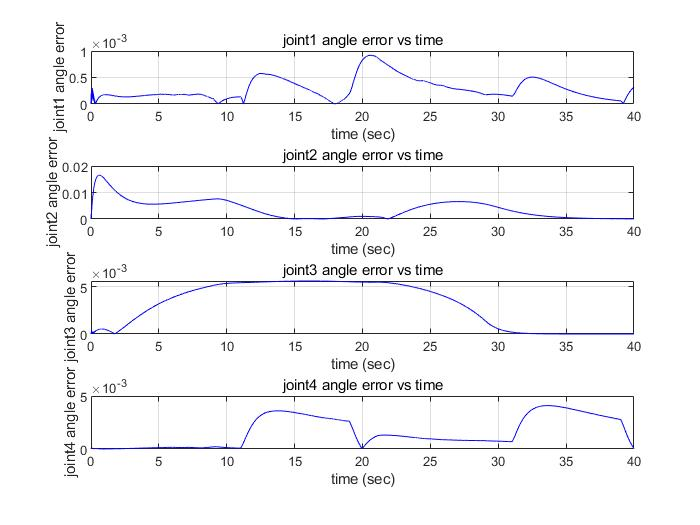
\includegraphics[width=8cm]{./fig/7.jpg}
    \caption{plastic modules of rectangular section}
    \label{f1}
\end{figure}

\section{Conclusion}

In conclusion, we successfully built the four-arm robot and achieve the function of welding in a specific area. We designed all the relevant data and reduced the errors by simulink. The maximum error in end effector position on the x and z axes is below 0.05, while the maximum error on the y axis is slightly over 0.10, and the largest error of joint angle is joint2 angle, and it just nearly reaches 0.02. These errors are far better than the standards set. Overall, we achieved the desired results. This is certainly a product worth buying and will bring unimaginable benefits to your company

%\section*{List of Symbols}
\begin{table}[H]
\centering
\begin{tabular}{lll}
 \toprule
  \textbf{Symbol}   &\textbf{Unit}      &\textbf{Explanation}\\
  \midrule
    n               & \si{\mole}        & Amount of substance \\
    m               & \si{\kilo\gram}   & Mass \\
    H               & \si{\kilo\joule\per\mole} & Molar enthalpy \\
    S               & \si{\joule\per\kelvin\per\mole}   & Molar entropy \\
    G               & \si{\kilo\joule\per\mole} & Gibbs free energy \\
    A               & \si{\kilo\joule\per\mole} & Helmholtz free energy \\
  \bottomrule
  \end{tabular}
\end{table}

%%%%%%%%%%%%%%%%%%%%%%%%%%%%%%%%%%%%%%%%%%%%%%%%%%%%%%%%%%
% Bibliography
%\newpage
%\bibliographystyle{IEEEtran}
%\bibliography{mendeley.bib}
%%%%%%%%%%%%%%%%%%%%%%%%%%%%%%%%%%%%%%%%%%%%%%%%%%%%%%%%%%
% Appendix
%\appendix
%\pagenumbering{roman}
%\section{First Appendix}
\label{app:first_appendix}
%\section{Second Appendix}
%\section{Third Appendix}
\end{document}
